\documentclass[tikz,border=2pt]{standalone}
\usepackage{newtxtext,newtxmath}
\begin{document}
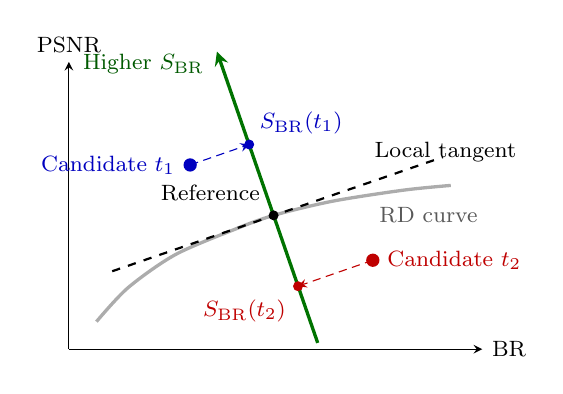
\begin{tikzpicture}[font=\footnotesize,>=stealth]
\draw[->] (0,0) -- (5.25,0) node[right] {BR};
\draw[->] (0,0) -- (0,3.65) node[above] {PSNR};
\draw[very thick,gray!65] plot[smooth] coordinates {(0.35,0.35) (0.75,0.78) (1.35,1.20) (2.10,1.52) (2.60,1.70) (3.35,1.88) (4.25,2.02) (4.85,2.08)};
\node[anchor=north west,text=gray!70!black] at (3.82,1.92) {RD curve};
\coordinate (reference) at (2.60,1.70);
\coordinate (candidateA) at (1.54,2.34);
\coordinate (projectionA) at (2.29,2.60);
\coordinate (candidateB) at (3.86,1.13);
\coordinate (projectionB) at (2.91,0.80);
\draw[dashed,thick] (0.55,0.99) -- (4.75,2.44);
\node[anchor=west] at (3.76,2.50) {Local tangent};
\draw[->,very thick,green!45!black] (3.16,0.08) -- (1.88,3.78);
\node[anchor=east,align=right,text=green!35!black] at (1.84,3.62) {Higher $S_{\mathrm{BR}}$};
\draw[->,densely dashed,blue!75!black] (candidateA) -- (projectionA);
\draw[->,densely dashed,red!75!black] (candidateB) -- (projectionB);
\fill[blue!75!black] (candidateA) circle (2.4pt);
\fill[red!75!black] (candidateB) circle (2.4pt);
\fill[blue!75!black] (projectionA) circle (1.8pt);
\fill[red!75!black] (projectionB) circle (1.8pt);
\fill[black] (reference) circle (1.8pt);
\node[anchor=east,text=blue!75!black] at (1.47,2.34) {Candidate $t_1$};
\node[anchor=west,text=red!75!black] at (3.92,1.13) {Candidate $t_2$};
\node[anchor=south west,text=blue!75!black] at (2.30,2.61) {$S_{\mathrm{BR}}(t_1)$};
\node[anchor=north east,text=red!75!black] at (2.88,0.75) {$S_{\mathrm{BR}}(t_2)$};
\node[anchor=south east] at (2.55,1.76) {Reference};
\end{tikzpicture}
\end{document}
